\documentclass[a4paper,12pt,twocolumn]{article}
\usepackage{graphicx}
\usepackage[margin=0.5in]{geometry}
\usepackage[cmex10]{amsmath}
\usepackage{array}
\usepackage{gensymb}
\usepackage{booktabs}
\title{Line Assignment}

\author{Ravi Sumanth Muppana- FWC22003}
\date{September 2022}
\providecommand{\norm}[1]{\left\lVert#1\right\rVert}
\providecommand{\abs}[1]{\left\vert#1\right\vert}
\let\vec\mathbf
\newcommand{\myvec}[1]{\ensuremath{\begin{pmatrix}#1\end{pmatrix}}}	
\newcommand{\mydet}[1]{\ensuremath{\begin{vmatrix}#1\end{vmatrix}}}
\providecommand{\brak}[1]{\ensuremath{\left((#1\right)}}
\begin{document}
\maketitle
\section{Problem:}
Show that if the diagonals of a quadrilateral bisect each other at right angles, then it is a rhombus
\maketitle
\section{Solution:}
\begin{figure}[h]
	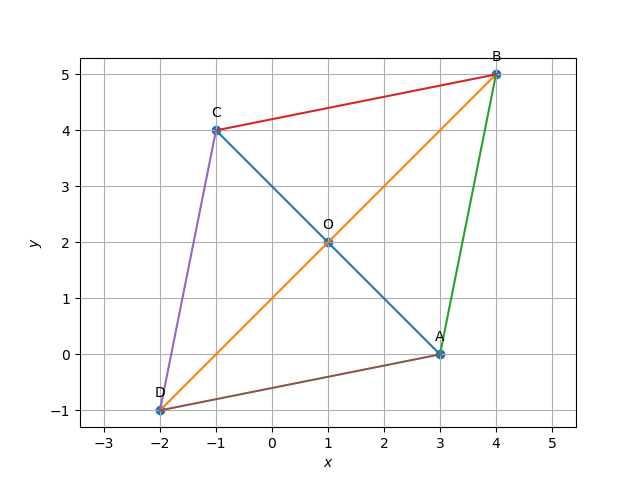
\includegraphics[width=\linewidth]{rhombus.png}
	\caption{Rhombus}
\end{figure}
\subsection{Theory:}
Let us assume two vectors $\vec{a}$ and $\vec{b}$ for sides $BA$ and $CB$. The diagonals $AC,BD$ are the addition and subtraction of the two vectors:
\begin{align}
	&\vec{(B-A)} = \vec{a}\\
	&\vec{(C-B)} = \vec{b}\\
	&\vec{(C-A)} = \vec{(C-B)} +\vec{(B-A)}\\
	&\vec{(C-A)} = \vec{b+a}\\
	&\vec{(D-B)} = \vec{b-a}\\
\end{align}
\subsection{Mathematical Calculation:}
Let the two diagonals be $\vec{a+b}$, $\vec{b-a}$. Since the diagonals are at right angle to each other,
\begin{align}
&0 = \vec{(a+b)^T}\vec{(b-a)}\\	
&||\vec{b}||^2 - ||\vec{a}||^2 = 0\\
&||\vec{b}|| = ||\vec{a}||\\
\end{align}
Hence, the two sides of the quadrilateral are equal. We need to prove the third side is also equal.
Now,
In triangle BOA and AOD;
\begin{align}
	&\vec{B-O} = \vec{p}\\
	&\vec{D-O} = \vec{-p}\\
	&\vec{A-O} = \vec{r}\\
\end{align}
\begin{align}
	&\vec{a} = \vec{(B-O)} - \vec{(A-O)}\\ 
	&\vec{d} = \vec{(D-O)} - \vec{(A-O)}\\
&||\vec{a}||^2 = ||\vec{p}||^2 + ||\vec{r}||^2 - 2\vec{p^Tr}\\
&||\vec{d}||^2 = ||\vec{-p}||^2 + ||\vec{r}||^2 + 2\vec{p^Tr}\\
\end{align}
The terms $\vec{p^Tr}$ is equal to zero as they is perpendicular.Therefore,
\begin{align}
	&||\vec{a}||^2 = ||\vec{p}||^2 + ||\vec{r}||^2\\
	&||\vec{d}||^2 = ||\vec{p}||^2 + ||\vec{r}||^2\\
	&Clearly, ||\vec{a}|| = ||\vec{d}||\\
\end{align}
Hence, all three sides are equal, it's a parallelogram. A parallelogram with it's diagonals as perpendicular bisectors is a rhombus.
\section{Construction:}
Consider any  three vertices of the rhombus. Using the vertices, find the midpoint of the diagonals, then find the fourth point using the midpoint and remaining vertex. 
\begin{table}[h]
	\centering
\setlength\extrarowheight{2pt}
	\begin{tabular}{|c|c|c|}
		\hline
		\textbf{variable} & \textbf{length/point} & \textbf{Description}\\
		\hline
		A & [3,0] & Vertex A\\
		\hline
		B & [4,5] & Vertex B\\
		\hline
		C & [-1,4] & Vertex C\\
		\hline                   
		D & [D-x,D-y] & Vertex D\\
		\hline
		M & (A+B)/2 & midpoint\\
		\hline
		(D-x,D-y) & (2*M[0]-B[0],2*M[1]-B[1]) & vertex of D\\
		\hline
	\end{tabular}
\end{table}

\end{document}
